%--------------------------------------------------------------------------------------------------------------
% kapitel/iststand.tex
%--------------------------------------------------------------------------------------------------------------

\chapter{Ist-Stand-Analyse}
In diesem Kapitel soll der Datenübernahmeprozess der SIV.AG analysiert werden. Um einen Einblick über den Ablauf zu erhalten wurden mehrere Bezugsquellen herangezogen. Zu den zählten die interne Dokumentation „Handbuch Datenmigration“ (nur für den internen Gebrauch), Beispieldaten und die dazu gehörigen SQL-Skripte aus vergangenen Datenmigrationsprojekten sowie Befragungen der Mitarbeiter aus der Abteilung  Datenmigration.

\section{Datenmigrationsprozess}
Gründe für eine Datenmigration durch SIV.AG können vielfältig sein. Zum einen kann der Kunde ein eigenentwickeltes \acrshort{erp}-System haben, welches nicht mehr den Anforderungen entspricht, bezogen auf gesetzliche oder organisatorische Aufgaben. Auf der anderen Seiten existiert noch kein \acrshort{erp}-System und es wird eins benötigt um diese Aufgaben umzusetzen. Des Weiteren könnte ein Kunde eine Standardsoftware z.\,B. von SAP, Schleupen oder Wilken besitzen und diese ablösen. Gründe dafür wären beispielsweise Kosten zu sparen durch ein preiswertes \acrshort{erp}-System oder eine Fusion zweier Unternehmen mit Unterschiedlichen Systemen von dem nur noch kVASy$^\text{\textregistered}$ verwendet wird. Gleichzeitig zur Datenmigration erfolgt eine Einführung in die kVASy$^\text{\textregistered}$-Software. Da kVASy$^\text{\textregistered}$ eine Standardsoftware ist wird eine Anpassung der Kundenwünsche nur in bestimmten Fälle vorgenommen. Im Normalfall wird das Zielsystem kVASy$^\text{\textregistered}$ nicht an den Daten des Kunden ausgerichtet, sondern es werden die Daten so transformiert das sie im Zielsystem verwendet werden können.
In der Abbildung \ref{pic:mig:end} wird ein allgemeiner Ablauf der Datenmigration durch die SIV.AG dargestellt.
\begin{figure}[ht]
	\begin{center}
		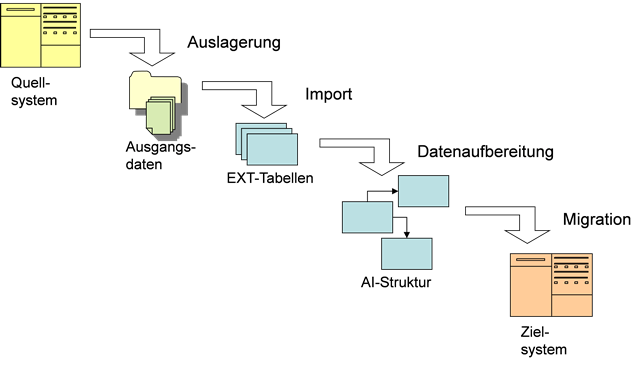
\includegraphics[scale=0.6]{bilder/migrationsverfahren.png}
		\caption{Migrationsverfahren durch die SIV.AG}
		\label{pic:mig:end}
	\end{center}
\end{figure}

Anhand der folgenden Teilschritte soll der Ablauf der Datenmigration, wie er durch die SIV.AG umgesetzt wird erläutert werden \cite{SIV11}:
\begin{itemize}
  \item Auslieferung und Laden der Testdaten
  \item Datenanalyse auf Basis von Testdaten
  \item Erstellung individueller Spezifikationen
  \item Definition der Übernahmeroutinen
  \item Durchführung der Testdatenkonvertierung
  \item Kontrolle der Testdaten durch Funktionstests
  \item Spezifikation der Echtdatenmigration
  \item Durchführung der Echtdatenübernahme
  \item Kontrolle und Bearbeitung der Echtdaten
  \item Abnahme des Konvertierungsverfahren
\end{itemize}

Wie in Kapitel 444 beschrieben wurde, gibt es für die Umsetzung einer Datenmigration mehrere Ansätze. Um dies zu bewerkstelligen verfolgt die SIV.AG den Big-Bang-Ansatz.

\subsection*{Auslieferung und Laden der Testdaten}
Bevor es zu einer Datenanalyse kommt müssen die Testdaten des Kunden vorliegen. Die Lieferung der Testdaten, nach Möglichkeit die gesamten Nutzdaten, erfolgt entweder durch den Kunden selber oder ein externes Unternehmen wird durch ihn beauftragt. In besonderen Fällen bietet die SIV.AG seine Hilfestellung in Form einer Beratung oder einer technischen Unterstützung an. Die Originaldaten müssen in einer elektronischen Form vorliegen wie z.\,B. Excel-Tabellen, Listen, \acrfull{csv}-Dateien oder Datenbankexports, obendrein muss eine Beschreibung der Daten mitgeliefert werden. Ausschlaggebend ist das die Daten in ein \acrshort{csv}-Format konvertierbar sind, um sie in eine Oracle-Datenbank zu importieren.
Ausschlaggebend für den Einsatz des \acrshort{csv}-Formats sind deren Eigenschaften zu den zählen unter anderem:
\begin{itemize}
  \item in der ersten Zeile der \acrshort{csv}-Datei stehen die Spaltennamen
  \item genau ein Datensatz pro Zeile 
  \item die Daten sind durch ein Semikolon im Datensatz getrennt
\end{itemize}
Für das Einlesen der Test- und Echtdatenübernahme  können folgende Datenträger verwendet werden \acrshort{cdrom}, \acrshort{dvd}, \acrshort{usb}-Festplatte, \acrshort{ftp}, \acrshort{https} und \acrshort{ssl}. Die Datenübernahme in die Oracle-Datenbank wird durch den SQL*Loader realisiert. Der SQL*Loaders benötigt für die Ausführung 2 Dateien. Zum einen die Datei mit den Originaldaten sowie einer Steuerdatei, welche den Aufbau und die Besonderheiten von Datendateien beschreibt. Die Steuerdatei kann eine einfache Textdatei sein. In dem Fall der Datenübernahme durch die SIV.AG wird als Steuerdatei eine Datei mit der Endung .td verwendet. Im Anhang \ref{pic:DTD:end} ist ein Beispiel einer solchen \acrfull{td} Datei zusehen. Zusätzlich erzeugt der SQL*Loader eine Bad-Datei sowie eine Log-Datei. Die Bad-Datei ist eine Fehler-Datei, in der eine Auflistung der erzeugten Fehler dargestellt werden. Ein Fehler könnte beispielsweise sein, dass der Datentyp nicht korrekt ist, mit dem Feld des zu übernehmenden Datensatzes. Die Log-Datei (auch Ergebnisprotokolldatei genannt) enthält das Protokoll über sämtliche Aktionen die bei der Datenübernahme durchgeführt worden sind z.\,B. Anzahl der übernommen Datensätze. Für die Übersichtlichkeit werden die Originaltabellen nicht eins zu eins übernommen, sondern es werden die Originaltabellennamen mit dem Präfix \textit{\textbf{EXT\_}} versehen, bevor sie in die Datenbank geschoben werden. Ein wichtiger Aspekt dabei ist die Überprüfung der Originaldaten der Kunden und der Aufbereiteten Originaldaten in Form des \textit{\textbf{EXT\_}} Präfixes, da dieses nicht automatisch überwacht wird. Diese Sache ist genau zu kontrollieren, damit keine Daten verloren oder geändert werden. Bekannte Probleme sind Umlautkonvertierung, Fehlen des letzten Datensatzes oder Abschneiden von Werten. Deshalb muss die Anzahl der Aufbereiteten Originaldaten in jedem Fall mit den Originaldaten korrespondieren. Zu dem müssen noch gewisse Voraussetzungen gegeben sein. Zum einen das Aufsetzen eines Testsystems durch den Kunden, welches für den Zeitraum der Migration nicht veränderbar ist. Die zweite Voraussetzung ist ein Gastzugang mit Leserechten auf das Testsystem.

\subsection*{Datenanalyse auf Basis von Testdaten}
Nach dem der komplette Dump (Speicherauszug) vorliegt kann die Analyse durch einen Consultant (Berater) durchgeführt werden. Die Seite des Zielsystems braucht nicht analysiert werden, da es bereits bekannt ist. Es sei denn es sollte ein Patch oder Update von kVASy$^\text{\textregistered}$ erfolgen, in dem z.\,B. ein neues Pflichtfeld eingeführt oder gelöscht wird. Die Herausforderung bei einer Datenmigration ist die Datenstruktur des Quellsystems herauszufinden, bzw. wie sie untereinander zusammenhängt. Ziel- und Quellsystem bilden zwar die gleichen Bereiche in der Energie- und Wasserwirtschaft ab, dennoch sind sie divergent. Die beiden System besitzen Felder mit Namen, Zähler, Adressen, Kundennummer, etc., aber trotzdem sind sie nicht homogen, weil beide System unabhängig von einander entwickelt worden sind. Um dem Consultant seine Arbeit zu erleichtern, wird zu den Originaldaten eine Dokumentation verlangt, um einen detaillierten Zusammenhang der Originaldaten zu bekommen. Die Übergabe eine Dokumentation ist, aber nicht als Pflicht anzusehen. Gründe dafür wären beispielsweise, dass der Kunde gar keinen Einblick in seine Daten hat, weil er sich mit ihnen nicht ausführlich auseinander gesetzt hat oder die Daten werden durch ein externes Unternehmen verwaltet. Der Grund bei einem externen Unternehmen ist auf seine Geheimhaltung der Datenbankstruktur zurückzuführen. In solchen Fällen wird eine Analyse um einiges erschwert und es kommt unweigerlich zu einem Mehraufwand.

\section{Transformationen}
\section{Qualitätskontrolle/Protokollierung}
\section{Ablaufsteuerung}
